% Created by tikzDevice version 0.12.3.1 on 2023-04-20 20:37:24
% !TEX encoding = UTF-8 Unicode
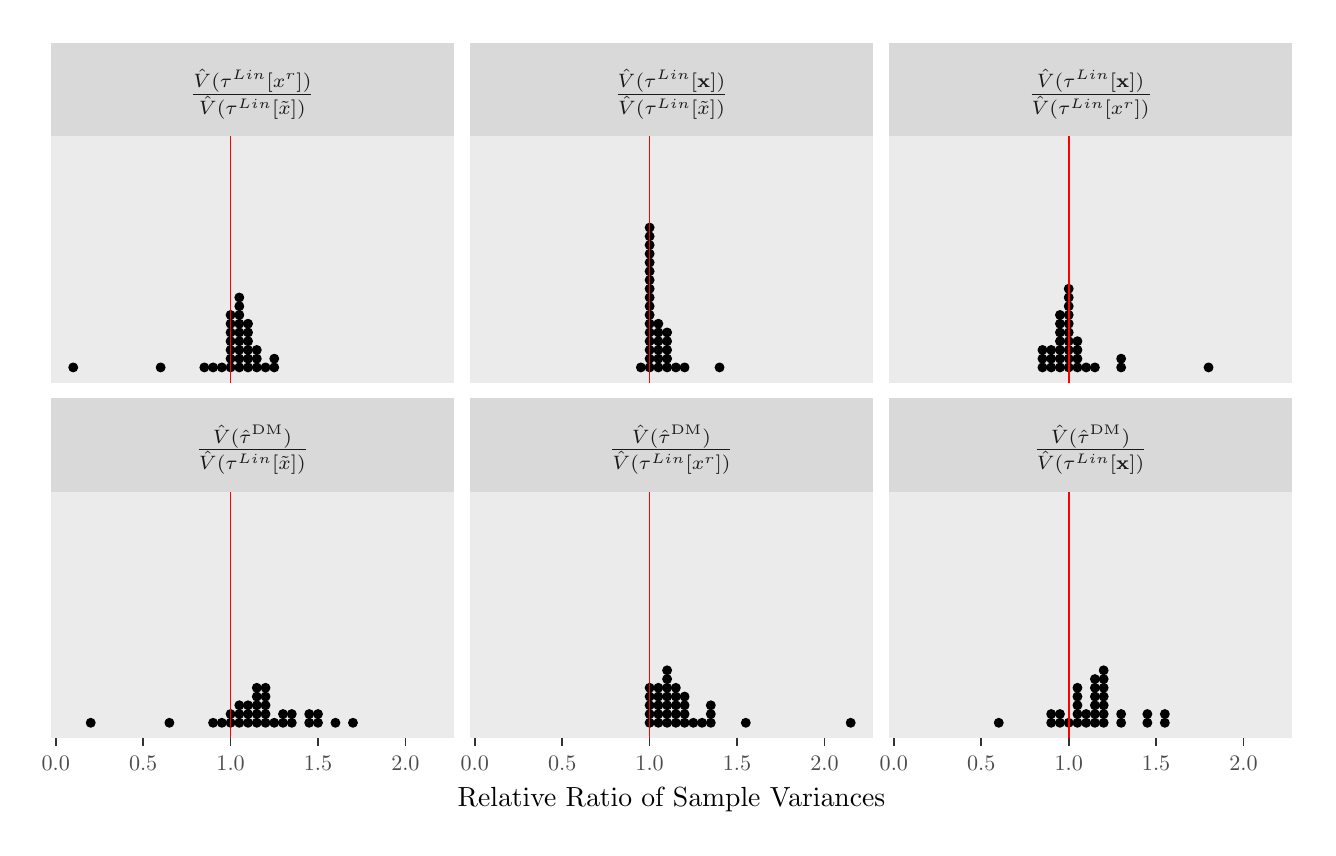
\begin{tikzpicture}[x=1pt,y=1pt]
\definecolor{fillColor}{RGB}{255,255,255}
\path[use as bounding box,fill=fillColor,fill opacity=0.00] (0,0) rectangle (462.53,289.08);
\begin{scope}
\path[clip] (  0.00,  0.00) rectangle (462.53,289.08);
\definecolor{drawColor}{RGB}{255,255,255}
\definecolor{fillColor}{RGB}{255,255,255}

\path[draw=drawColor,line width= 0.6pt,line join=round,line cap=round,fill=fillColor] (  0.00,  0.00) rectangle (462.53,289.08);
\end{scope}
\begin{scope}
\path[clip] (  8.25,160.68) rectangle (154.18,249.78);
\definecolor{fillColor}{gray}{0.92}

\path[fill=fillColor] (  8.25,160.68) rectangle (154.18,249.78);
\definecolor{drawColor}{RGB}{0,0,0}
\definecolor{fillColor}{RGB}{0,0,0}

\path[draw=drawColor,line width= 0.4pt,line join=round,fill=fillColor] ( 16.46,166.31) circle (  1.58);

\path[draw=drawColor,line width= 0.4pt,line join=round,fill=fillColor] ( 48.05,166.31) circle (  1.58);

\path[draw=drawColor,line width= 0.4pt,line join=round,fill=fillColor] ( 63.84,166.31) circle (  1.58);

\path[draw=drawColor,line width= 0.4pt,line join=round,fill=fillColor] ( 67.00,166.31) circle (  1.58);

\path[draw=drawColor,line width= 0.4pt,line join=round,fill=fillColor] ( 70.16,166.31) circle (  1.58);

\path[draw=drawColor,line width= 0.4pt,line join=round,fill=fillColor] ( 73.32,166.31) circle (  1.58);

\path[draw=drawColor,line width= 0.4pt,line join=round,fill=fillColor] ( 73.32,169.47) circle (  1.58);

\path[draw=drawColor,line width= 0.4pt,line join=round,fill=fillColor] ( 73.32,172.62) circle (  1.58);

\path[draw=drawColor,line width= 0.4pt,line join=round,fill=fillColor] ( 73.32,175.78) circle (  1.58);

\path[draw=drawColor,line width= 0.4pt,line join=round,fill=fillColor] ( 73.32,178.94) circle (  1.58);

\path[draw=drawColor,line width= 0.4pt,line join=round,fill=fillColor] ( 73.32,182.10) circle (  1.58);

\path[draw=drawColor,line width= 0.4pt,line join=round,fill=fillColor] ( 73.32,185.26) circle (  1.58);

\path[draw=drawColor,line width= 0.4pt,line join=round,fill=fillColor] ( 76.48,166.31) circle (  1.58);

\path[draw=drawColor,line width= 0.4pt,line join=round,fill=fillColor] ( 76.48,169.47) circle (  1.58);

\path[draw=drawColor,line width= 0.4pt,line join=round,fill=fillColor] ( 76.48,172.62) circle (  1.58);

\path[draw=drawColor,line width= 0.4pt,line join=round,fill=fillColor] ( 76.48,175.78) circle (  1.58);

\path[draw=drawColor,line width= 0.4pt,line join=round,fill=fillColor] ( 76.48,178.94) circle (  1.58);

\path[draw=drawColor,line width= 0.4pt,line join=round,fill=fillColor] ( 76.48,182.10) circle (  1.58);

\path[draw=drawColor,line width= 0.4pt,line join=round,fill=fillColor] ( 76.48,185.26) circle (  1.58);

\path[draw=drawColor,line width= 0.4pt,line join=round,fill=fillColor] ( 76.48,188.42) circle (  1.58);

\path[draw=drawColor,line width= 0.4pt,line join=round,fill=fillColor] ( 76.48,191.58) circle (  1.58);

\path[draw=drawColor,line width= 0.4pt,line join=round,fill=fillColor] ( 79.63,166.31) circle (  1.58);

\path[draw=drawColor,line width= 0.4pt,line join=round,fill=fillColor] ( 79.63,169.47) circle (  1.58);

\path[draw=drawColor,line width= 0.4pt,line join=round,fill=fillColor] ( 79.63,172.62) circle (  1.58);

\path[draw=drawColor,line width= 0.4pt,line join=round,fill=fillColor] ( 79.63,175.78) circle (  1.58);

\path[draw=drawColor,line width= 0.4pt,line join=round,fill=fillColor] ( 79.63,178.94) circle (  1.58);

\path[draw=drawColor,line width= 0.4pt,line join=round,fill=fillColor] ( 79.63,182.10) circle (  1.58);

\path[draw=drawColor,line width= 0.4pt,line join=round,fill=fillColor] ( 82.79,166.31) circle (  1.58);

\path[draw=drawColor,line width= 0.4pt,line join=round,fill=fillColor] ( 82.79,169.47) circle (  1.58);

\path[draw=drawColor,line width= 0.4pt,line join=round,fill=fillColor] ( 82.79,172.62) circle (  1.58);

\path[draw=drawColor,line width= 0.4pt,line join=round,fill=fillColor] ( 85.95,166.31) circle (  1.58);

\path[draw=drawColor,line width= 0.4pt,line join=round,fill=fillColor] ( 89.11,166.31) circle (  1.58);

\path[draw=drawColor,line width= 0.4pt,line join=round,fill=fillColor] ( 89.11,169.47) circle (  1.58);
\definecolor{drawColor}{RGB}{255,0,0}

\path[draw=drawColor,line width= 0.6pt,line join=round] ( 73.32,160.68) -- ( 73.32,249.78);
\end{scope}
\begin{scope}
\path[clip] (  8.25, 32.28) rectangle (154.18,121.38);
\definecolor{fillColor}{gray}{0.92}

\path[fill=fillColor] (  8.25, 32.28) rectangle (154.18,121.38);
\definecolor{drawColor}{RGB}{0,0,0}
\definecolor{fillColor}{RGB}{0,0,0}

\path[draw=drawColor,line width= 0.4pt,line join=round,fill=fillColor] ( 22.78, 37.90) circle (  1.58);

\path[draw=drawColor,line width= 0.4pt,line join=round,fill=fillColor] ( 51.21, 37.90) circle (  1.58);

\path[draw=drawColor,line width= 0.4pt,line join=round,fill=fillColor] ( 67.00, 37.90) circle (  1.58);

\path[draw=drawColor,line width= 0.4pt,line join=round,fill=fillColor] ( 70.16, 37.90) circle (  1.58);

\path[draw=drawColor,line width= 0.4pt,line join=round,fill=fillColor] ( 73.32, 37.90) circle (  1.58);

\path[draw=drawColor,line width= 0.4pt,line join=round,fill=fillColor] ( 73.32, 41.06) circle (  1.58);

\path[draw=drawColor,line width= 0.4pt,line join=round,fill=fillColor] ( 76.48, 37.90) circle (  1.58);

\path[draw=drawColor,line width= 0.4pt,line join=round,fill=fillColor] ( 76.48, 41.06) circle (  1.58);

\path[draw=drawColor,line width= 0.4pt,line join=round,fill=fillColor] ( 76.48, 44.22) circle (  1.58);

\path[draw=drawColor,line width= 0.4pt,line join=round,fill=fillColor] ( 79.63, 37.90) circle (  1.58);

\path[draw=drawColor,line width= 0.4pt,line join=round,fill=fillColor] ( 79.63, 41.06) circle (  1.58);

\path[draw=drawColor,line width= 0.4pt,line join=round,fill=fillColor] ( 79.63, 44.22) circle (  1.58);

\path[draw=drawColor,line width= 0.4pt,line join=round,fill=fillColor] ( 82.79, 37.90) circle (  1.58);

\path[draw=drawColor,line width= 0.4pt,line join=round,fill=fillColor] ( 82.79, 41.06) circle (  1.58);

\path[draw=drawColor,line width= 0.4pt,line join=round,fill=fillColor] ( 82.79, 44.22) circle (  1.58);

\path[draw=drawColor,line width= 0.4pt,line join=round,fill=fillColor] ( 82.79, 47.38) circle (  1.58);

\path[draw=drawColor,line width= 0.4pt,line join=round,fill=fillColor] ( 82.79, 50.54) circle (  1.58);

\path[draw=drawColor,line width= 0.4pt,line join=round,fill=fillColor] ( 85.95, 37.90) circle (  1.58);

\path[draw=drawColor,line width= 0.4pt,line join=round,fill=fillColor] ( 85.95, 41.06) circle (  1.58);

\path[draw=drawColor,line width= 0.4pt,line join=round,fill=fillColor] ( 85.95, 44.22) circle (  1.58);

\path[draw=drawColor,line width= 0.4pt,line join=round,fill=fillColor] ( 85.95, 47.38) circle (  1.58);

\path[draw=drawColor,line width= 0.4pt,line join=round,fill=fillColor] ( 85.95, 50.54) circle (  1.58);

\path[draw=drawColor,line width= 0.4pt,line join=round,fill=fillColor] ( 89.11, 37.90) circle (  1.58);

\path[draw=drawColor,line width= 0.4pt,line join=round,fill=fillColor] ( 92.27, 37.90) circle (  1.58);

\path[draw=drawColor,line width= 0.4pt,line join=round,fill=fillColor] ( 92.27, 41.06) circle (  1.58);

\path[draw=drawColor,line width= 0.4pt,line join=round,fill=fillColor] ( 95.43, 37.90) circle (  1.58);

\path[draw=drawColor,line width= 0.4pt,line join=round,fill=fillColor] ( 95.43, 41.06) circle (  1.58);

\path[draw=drawColor,line width= 0.4pt,line join=round,fill=fillColor] (101.74, 37.90) circle (  1.58);

\path[draw=drawColor,line width= 0.4pt,line join=round,fill=fillColor] (101.74, 41.06) circle (  1.58);

\path[draw=drawColor,line width= 0.4pt,line join=round,fill=fillColor] (104.90, 37.90) circle (  1.58);

\path[draw=drawColor,line width= 0.4pt,line join=round,fill=fillColor] (104.90, 41.06) circle (  1.58);

\path[draw=drawColor,line width= 0.4pt,line join=round,fill=fillColor] (111.22, 37.90) circle (  1.58);

\path[draw=drawColor,line width= 0.4pt,line join=round,fill=fillColor] (117.54, 37.90) circle (  1.58);
\definecolor{drawColor}{RGB}{255,0,0}

\path[draw=drawColor,line width= 0.6pt,line join=round] ( 73.32, 32.28) -- ( 73.32,121.38);
\end{scope}
\begin{scope}
\path[clip] (159.68,160.68) rectangle (305.60,249.78);
\definecolor{fillColor}{gray}{0.92}

\path[fill=fillColor] (159.68,160.68) rectangle (305.60,249.78);
\definecolor{drawColor}{RGB}{0,0,0}
\definecolor{fillColor}{RGB}{0,0,0}

\path[draw=drawColor,line width= 0.4pt,line join=round,fill=fillColor] (221.58,166.31) circle (  1.58);

\path[draw=drawColor,line width= 0.4pt,line join=round,fill=fillColor] (224.74,166.31) circle (  1.58);

\path[draw=drawColor,line width= 0.4pt,line join=round,fill=fillColor] (224.74,169.47) circle (  1.58);

\path[draw=drawColor,line width= 0.4pt,line join=round,fill=fillColor] (224.74,172.62) circle (  1.58);

\path[draw=drawColor,line width= 0.4pt,line join=round,fill=fillColor] (224.74,175.78) circle (  1.58);

\path[draw=drawColor,line width= 0.4pt,line join=round,fill=fillColor] (224.74,178.94) circle (  1.58);

\path[draw=drawColor,line width= 0.4pt,line join=round,fill=fillColor] (224.74,182.10) circle (  1.58);

\path[draw=drawColor,line width= 0.4pt,line join=round,fill=fillColor] (224.74,185.26) circle (  1.58);

\path[draw=drawColor,line width= 0.4pt,line join=round,fill=fillColor] (224.74,188.42) circle (  1.58);

\path[draw=drawColor,line width= 0.4pt,line join=round,fill=fillColor] (224.74,191.58) circle (  1.58);

\path[draw=drawColor,line width= 0.4pt,line join=round,fill=fillColor] (224.74,194.73) circle (  1.58);

\path[draw=drawColor,line width= 0.4pt,line join=round,fill=fillColor] (224.74,197.89) circle (  1.58);

\path[draw=drawColor,line width= 0.4pt,line join=round,fill=fillColor] (224.74,201.05) circle (  1.58);

\path[draw=drawColor,line width= 0.4pt,line join=round,fill=fillColor] (224.74,204.21) circle (  1.58);

\path[draw=drawColor,line width= 0.4pt,line join=round,fill=fillColor] (224.74,207.37) circle (  1.58);

\path[draw=drawColor,line width= 0.4pt,line join=round,fill=fillColor] (224.74,210.53) circle (  1.58);

\path[draw=drawColor,line width= 0.4pt,line join=round,fill=fillColor] (224.74,213.69) circle (  1.58);

\path[draw=drawColor,line width= 0.4pt,line join=round,fill=fillColor] (224.74,216.84) circle (  1.58);

\path[draw=drawColor,line width= 0.4pt,line join=round,fill=fillColor] (227.90,166.31) circle (  1.58);

\path[draw=drawColor,line width= 0.4pt,line join=round,fill=fillColor] (227.90,169.47) circle (  1.58);

\path[draw=drawColor,line width= 0.4pt,line join=round,fill=fillColor] (227.90,172.62) circle (  1.58);

\path[draw=drawColor,line width= 0.4pt,line join=round,fill=fillColor] (227.90,175.78) circle (  1.58);

\path[draw=drawColor,line width= 0.4pt,line join=round,fill=fillColor] (227.90,178.94) circle (  1.58);

\path[draw=drawColor,line width= 0.4pt,line join=round,fill=fillColor] (227.90,182.10) circle (  1.58);

\path[draw=drawColor,line width= 0.4pt,line join=round,fill=fillColor] (231.06,166.31) circle (  1.58);

\path[draw=drawColor,line width= 0.4pt,line join=round,fill=fillColor] (231.06,169.47) circle (  1.58);

\path[draw=drawColor,line width= 0.4pt,line join=round,fill=fillColor] (231.06,172.62) circle (  1.58);

\path[draw=drawColor,line width= 0.4pt,line join=round,fill=fillColor] (231.06,175.78) circle (  1.58);

\path[draw=drawColor,line width= 0.4pt,line join=round,fill=fillColor] (231.06,178.94) circle (  1.58);

\path[draw=drawColor,line width= 0.4pt,line join=round,fill=fillColor] (234.22,166.31) circle (  1.58);

\path[draw=drawColor,line width= 0.4pt,line join=round,fill=fillColor] (237.38,166.31) circle (  1.58);

\path[draw=drawColor,line width= 0.4pt,line join=round,fill=fillColor] (250.01,166.31) circle (  1.58);
\definecolor{drawColor}{RGB}{255,0,0}

\path[draw=drawColor,line width= 0.6pt,line join=round] (224.74,160.68) -- (224.74,249.78);
\end{scope}
\begin{scope}
\path[clip] (159.68, 32.28) rectangle (305.60,121.38);
\definecolor{fillColor}{gray}{0.92}

\path[fill=fillColor] (159.68, 32.28) rectangle (305.60,121.38);
\definecolor{drawColor}{RGB}{0,0,0}
\definecolor{fillColor}{RGB}{0,0,0}

\path[draw=drawColor,line width= 0.4pt,line join=round,fill=fillColor] (224.74, 37.90) circle (  1.58);

\path[draw=drawColor,line width= 0.4pt,line join=round,fill=fillColor] (224.74, 41.06) circle (  1.58);

\path[draw=drawColor,line width= 0.4pt,line join=round,fill=fillColor] (224.74, 44.22) circle (  1.58);

\path[draw=drawColor,line width= 0.4pt,line join=round,fill=fillColor] (224.74, 47.38) circle (  1.58);

\path[draw=drawColor,line width= 0.4pt,line join=round,fill=fillColor] (224.74, 50.54) circle (  1.58);

\path[draw=drawColor,line width= 0.4pt,line join=round,fill=fillColor] (227.90, 37.90) circle (  1.58);

\path[draw=drawColor,line width= 0.4pt,line join=round,fill=fillColor] (227.90, 41.06) circle (  1.58);

\path[draw=drawColor,line width= 0.4pt,line join=round,fill=fillColor] (227.90, 44.22) circle (  1.58);

\path[draw=drawColor,line width= 0.4pt,line join=round,fill=fillColor] (227.90, 47.38) circle (  1.58);

\path[draw=drawColor,line width= 0.4pt,line join=round,fill=fillColor] (227.90, 50.54) circle (  1.58);

\path[draw=drawColor,line width= 0.4pt,line join=round,fill=fillColor] (231.06, 37.90) circle (  1.58);

\path[draw=drawColor,line width= 0.4pt,line join=round,fill=fillColor] (231.06, 41.06) circle (  1.58);

\path[draw=drawColor,line width= 0.4pt,line join=round,fill=fillColor] (231.06, 44.22) circle (  1.58);

\path[draw=drawColor,line width= 0.4pt,line join=round,fill=fillColor] (231.06, 47.38) circle (  1.58);

\path[draw=drawColor,line width= 0.4pt,line join=round,fill=fillColor] (231.06, 50.54) circle (  1.58);

\path[draw=drawColor,line width= 0.4pt,line join=round,fill=fillColor] (231.06, 53.70) circle (  1.58);

\path[draw=drawColor,line width= 0.4pt,line join=round,fill=fillColor] (231.06, 56.86) circle (  1.58);

\path[draw=drawColor,line width= 0.4pt,line join=round,fill=fillColor] (234.22, 37.90) circle (  1.58);

\path[draw=drawColor,line width= 0.4pt,line join=round,fill=fillColor] (234.22, 41.06) circle (  1.58);

\path[draw=drawColor,line width= 0.4pt,line join=round,fill=fillColor] (234.22, 44.22) circle (  1.58);

\path[draw=drawColor,line width= 0.4pt,line join=round,fill=fillColor] (234.22, 47.38) circle (  1.58);

\path[draw=drawColor,line width= 0.4pt,line join=round,fill=fillColor] (234.22, 50.54) circle (  1.58);

\path[draw=drawColor,line width= 0.4pt,line join=round,fill=fillColor] (237.38, 37.90) circle (  1.58);

\path[draw=drawColor,line width= 0.4pt,line join=round,fill=fillColor] (237.38, 41.06) circle (  1.58);

\path[draw=drawColor,line width= 0.4pt,line join=round,fill=fillColor] (237.38, 44.22) circle (  1.58);

\path[draw=drawColor,line width= 0.4pt,line join=round,fill=fillColor] (237.38, 47.38) circle (  1.58);

\path[draw=drawColor,line width= 0.4pt,line join=round,fill=fillColor] (240.54, 37.90) circle (  1.58);

\path[draw=drawColor,line width= 0.4pt,line join=round,fill=fillColor] (243.69, 37.90) circle (  1.58);

\path[draw=drawColor,line width= 0.4pt,line join=round,fill=fillColor] (246.85, 37.90) circle (  1.58);

\path[draw=drawColor,line width= 0.4pt,line join=round,fill=fillColor] (246.85, 41.06) circle (  1.58);

\path[draw=drawColor,line width= 0.4pt,line join=round,fill=fillColor] (246.85, 44.22) circle (  1.58);

\path[draw=drawColor,line width= 0.4pt,line join=round,fill=fillColor] (259.49, 37.90) circle (  1.58);

\path[draw=drawColor,line width= 0.4pt,line join=round,fill=fillColor] (297.39, 37.90) circle (  1.58);
\definecolor{drawColor}{RGB}{255,0,0}

\path[draw=drawColor,line width= 0.6pt,line join=round] (224.74, 32.28) -- (224.74,121.38);
\end{scope}
\begin{scope}
\path[clip] (311.10,160.68) rectangle (457.03,249.78);
\definecolor{fillColor}{gray}{0.92}

\path[fill=fillColor] (311.10,160.68) rectangle (457.03,249.78);
\definecolor{drawColor}{RGB}{0,0,0}
\definecolor{fillColor}{RGB}{0,0,0}

\path[draw=drawColor,line width= 0.4pt,line join=round,fill=fillColor] (366.69,166.31) circle (  1.58);

\path[draw=drawColor,line width= 0.4pt,line join=round,fill=fillColor] (366.69,169.47) circle (  1.58);

\path[draw=drawColor,line width= 0.4pt,line join=round,fill=fillColor] (366.69,172.62) circle (  1.58);

\path[draw=drawColor,line width= 0.4pt,line join=round,fill=fillColor] (369.85,166.31) circle (  1.58);

\path[draw=drawColor,line width= 0.4pt,line join=round,fill=fillColor] (369.85,169.47) circle (  1.58);

\path[draw=drawColor,line width= 0.4pt,line join=round,fill=fillColor] (369.85,172.62) circle (  1.58);

\path[draw=drawColor,line width= 0.4pt,line join=round,fill=fillColor] (373.01,166.31) circle (  1.58);

\path[draw=drawColor,line width= 0.4pt,line join=round,fill=fillColor] (373.01,169.47) circle (  1.58);

\path[draw=drawColor,line width= 0.4pt,line join=round,fill=fillColor] (373.01,172.62) circle (  1.58);

\path[draw=drawColor,line width= 0.4pt,line join=round,fill=fillColor] (373.01,175.78) circle (  1.58);

\path[draw=drawColor,line width= 0.4pt,line join=round,fill=fillColor] (373.01,178.94) circle (  1.58);

\path[draw=drawColor,line width= 0.4pt,line join=round,fill=fillColor] (373.01,182.10) circle (  1.58);

\path[draw=drawColor,line width= 0.4pt,line join=round,fill=fillColor] (373.01,185.26) circle (  1.58);

\path[draw=drawColor,line width= 0.4pt,line join=round,fill=fillColor] (376.17,166.31) circle (  1.58);

\path[draw=drawColor,line width= 0.4pt,line join=round,fill=fillColor] (376.17,169.47) circle (  1.58);

\path[draw=drawColor,line width= 0.4pt,line join=round,fill=fillColor] (376.17,172.62) circle (  1.58);

\path[draw=drawColor,line width= 0.4pt,line join=round,fill=fillColor] (376.17,175.78) circle (  1.58);

\path[draw=drawColor,line width= 0.4pt,line join=round,fill=fillColor] (376.17,178.94) circle (  1.58);

\path[draw=drawColor,line width= 0.4pt,line join=round,fill=fillColor] (376.17,182.10) circle (  1.58);

\path[draw=drawColor,line width= 0.4pt,line join=round,fill=fillColor] (376.17,185.26) circle (  1.58);

\path[draw=drawColor,line width= 0.4pt,line join=round,fill=fillColor] (376.17,188.42) circle (  1.58);

\path[draw=drawColor,line width= 0.4pt,line join=round,fill=fillColor] (376.17,191.58) circle (  1.58);

\path[draw=drawColor,line width= 0.4pt,line join=round,fill=fillColor] (376.17,194.73) circle (  1.58);

\path[draw=drawColor,line width= 0.4pt,line join=round,fill=fillColor] (379.33,166.31) circle (  1.58);

\path[draw=drawColor,line width= 0.4pt,line join=round,fill=fillColor] (379.33,169.47) circle (  1.58);

\path[draw=drawColor,line width= 0.4pt,line join=round,fill=fillColor] (379.33,172.62) circle (  1.58);

\path[draw=drawColor,line width= 0.4pt,line join=round,fill=fillColor] (379.33,175.78) circle (  1.58);

\path[draw=drawColor,line width= 0.4pt,line join=round,fill=fillColor] (382.49,166.31) circle (  1.58);

\path[draw=drawColor,line width= 0.4pt,line join=round,fill=fillColor] (385.64,166.31) circle (  1.58);

\path[draw=drawColor,line width= 0.4pt,line join=round,fill=fillColor] (395.12,166.31) circle (  1.58);

\path[draw=drawColor,line width= 0.4pt,line join=round,fill=fillColor] (395.12,169.47) circle (  1.58);

\path[draw=drawColor,line width= 0.4pt,line join=round,fill=fillColor] (426.71,166.31) circle (  1.58);
\definecolor{drawColor}{RGB}{255,0,0}

\path[draw=drawColor,line width= 0.6pt,line join=round] (376.17,160.68) -- (376.17,249.78);
\end{scope}
\begin{scope}
\path[clip] (311.10, 32.28) rectangle (457.03,121.38);
\definecolor{fillColor}{gray}{0.92}

\path[fill=fillColor] (311.10, 32.28) rectangle (457.03,121.38);
\definecolor{drawColor}{RGB}{0,0,0}
\definecolor{fillColor}{RGB}{0,0,0}

\path[draw=drawColor,line width= 0.4pt,line join=round,fill=fillColor] (350.90, 37.90) circle (  1.58);

\path[draw=drawColor,line width= 0.4pt,line join=round,fill=fillColor] (369.85, 37.90) circle (  1.58);

\path[draw=drawColor,line width= 0.4pt,line join=round,fill=fillColor] (369.85, 41.06) circle (  1.58);

\path[draw=drawColor,line width= 0.4pt,line join=round,fill=fillColor] (373.01, 37.90) circle (  1.58);

\path[draw=drawColor,line width= 0.4pt,line join=round,fill=fillColor] (373.01, 41.06) circle (  1.58);

\path[draw=drawColor,line width= 0.4pt,line join=round,fill=fillColor] (376.17, 37.90) circle (  1.58);

\path[draw=drawColor,line width= 0.4pt,line join=round,fill=fillColor] (379.33, 37.90) circle (  1.58);

\path[draw=drawColor,line width= 0.4pt,line join=round,fill=fillColor] (379.33, 41.06) circle (  1.58);

\path[draw=drawColor,line width= 0.4pt,line join=round,fill=fillColor] (379.33, 44.22) circle (  1.58);

\path[draw=drawColor,line width= 0.4pt,line join=round,fill=fillColor] (379.33, 47.38) circle (  1.58);

\path[draw=drawColor,line width= 0.4pt,line join=round,fill=fillColor] (379.33, 50.54) circle (  1.58);

\path[draw=drawColor,line width= 0.4pt,line join=round,fill=fillColor] (382.49, 37.90) circle (  1.58);

\path[draw=drawColor,line width= 0.4pt,line join=round,fill=fillColor] (382.49, 41.06) circle (  1.58);

\path[draw=drawColor,line width= 0.4pt,line join=round,fill=fillColor] (385.64, 37.90) circle (  1.58);

\path[draw=drawColor,line width= 0.4pt,line join=round,fill=fillColor] (385.64, 41.06) circle (  1.58);

\path[draw=drawColor,line width= 0.4pt,line join=round,fill=fillColor] (385.64, 44.22) circle (  1.58);

\path[draw=drawColor,line width= 0.4pt,line join=round,fill=fillColor] (385.64, 47.38) circle (  1.58);

\path[draw=drawColor,line width= 0.4pt,line join=round,fill=fillColor] (385.64, 50.54) circle (  1.58);

\path[draw=drawColor,line width= 0.4pt,line join=round,fill=fillColor] (385.64, 53.70) circle (  1.58);

\path[draw=drawColor,line width= 0.4pt,line join=round,fill=fillColor] (388.80, 37.90) circle (  1.58);

\path[draw=drawColor,line width= 0.4pt,line join=round,fill=fillColor] (388.80, 41.06) circle (  1.58);

\path[draw=drawColor,line width= 0.4pt,line join=round,fill=fillColor] (388.80, 44.22) circle (  1.58);

\path[draw=drawColor,line width= 0.4pt,line join=round,fill=fillColor] (388.80, 47.38) circle (  1.58);

\path[draw=drawColor,line width= 0.4pt,line join=round,fill=fillColor] (388.80, 50.54) circle (  1.58);

\path[draw=drawColor,line width= 0.4pt,line join=round,fill=fillColor] (388.80, 53.70) circle (  1.58);

\path[draw=drawColor,line width= 0.4pt,line join=round,fill=fillColor] (388.80, 56.86) circle (  1.58);

\path[draw=drawColor,line width= 0.4pt,line join=round,fill=fillColor] (395.12, 37.90) circle (  1.58);

\path[draw=drawColor,line width= 0.4pt,line join=round,fill=fillColor] (395.12, 41.06) circle (  1.58);

\path[draw=drawColor,line width= 0.4pt,line join=round,fill=fillColor] (404.60, 37.90) circle (  1.58);

\path[draw=drawColor,line width= 0.4pt,line join=round,fill=fillColor] (404.60, 41.06) circle (  1.58);

\path[draw=drawColor,line width= 0.4pt,line join=round,fill=fillColor] (410.91, 37.90) circle (  1.58);

\path[draw=drawColor,line width= 0.4pt,line join=round,fill=fillColor] (410.91, 41.06) circle (  1.58);
\definecolor{drawColor}{RGB}{255,0,0}

\path[draw=drawColor,line width= 0.6pt,line join=round] (376.17, 32.28) -- (376.17,121.38);
\end{scope}
\begin{scope}
\path[clip] (  8.25,121.38) rectangle (154.18,155.18);
\definecolor{fillColor}{gray}{0.85}

\path[fill=fillColor] (  8.25,121.38) rectangle (154.18,155.18);
\definecolor{drawColor}{gray}{0.10}

\node[text=drawColor,anchor=base,inner sep=0pt, outer sep=0pt, scale=  1.00] at ( 81.21,141.35) {};

\node[text=drawColor,anchor=base,inner sep=0pt, outer sep=0pt, scale=  1.00] at ( 81.21,134.15) {$\frac{\hat{\mathbb{V}}(\hat{\tau}^{\mathrm{DM}})}{\hat{\mathbb{V}}(\tau^{Lin}[\tilde{x}])}$};

\node[text=drawColor,anchor=base,inner sep=0pt, outer sep=0pt, scale=  1.00] at ( 81.21,126.95) {};
\end{scope}
\begin{scope}
\path[clip] (159.68,121.38) rectangle (305.60,155.18);
\definecolor{fillColor}{gray}{0.85}

\path[fill=fillColor] (159.68,121.38) rectangle (305.60,155.18);
\definecolor{drawColor}{gray}{0.10}

\node[text=drawColor,anchor=base,inner sep=0pt, outer sep=0pt, scale=  1.00] at (232.64,141.35) {};

\node[text=drawColor,anchor=base,inner sep=0pt, outer sep=0pt, scale=  1.00] at (232.64,134.15) {$\frac{\hat{\mathbb{V}}(\hat{\tau}^{\mathrm{DM}})}{\hat{\mathbb{V}}(\tau^{Lin}[x^r])}$};

\node[text=drawColor,anchor=base,inner sep=0pt, outer sep=0pt, scale=  1.00] at (232.64,126.95) {};
\end{scope}
\begin{scope}
\path[clip] (311.10,121.38) rectangle (457.03,155.18);
\definecolor{fillColor}{gray}{0.85}

\path[fill=fillColor] (311.10,121.38) rectangle (457.03,155.18);
\definecolor{drawColor}{gray}{0.10}

\node[text=drawColor,anchor=base,inner sep=0pt, outer sep=0pt, scale=  1.00] at (384.06,141.35) {};

\node[text=drawColor,anchor=base,inner sep=0pt, outer sep=0pt, scale=  1.00] at (384.06,134.15) {$\frac{\hat{\mathbb{V}}(\hat{\tau}^{\mathrm{DM}})}{\hat{\mathbb{V}}(\tau^{Lin}[\mathbf{x}])}$};

\node[text=drawColor,anchor=base,inner sep=0pt, outer sep=0pt, scale=  1.00] at (384.06,126.95) {};
\end{scope}
\begin{scope}
\path[clip] (  8.25,249.78) rectangle (154.18,283.58);
\definecolor{fillColor}{gray}{0.85}

\path[fill=fillColor] (  8.25,249.78) rectangle (154.18,283.58);
\definecolor{drawColor}{gray}{0.10}

\node[text=drawColor,anchor=base,inner sep=0pt, outer sep=0pt, scale=  1.00] at ( 81.21,269.75) {};

\node[text=drawColor,anchor=base,inner sep=0pt, outer sep=0pt, scale=  1.00] at ( 81.21,262.55) {$\frac{\hat{\mathbb{V}}(\tau^{Lin}[x^r])}{\hat{\mathbb{V}}(\tau^{Lin}[\tilde{x}])}$};

\node[text=drawColor,anchor=base,inner sep=0pt, outer sep=0pt, scale=  1.00] at ( 81.21,255.35) {};
\end{scope}
\begin{scope}
\path[clip] (159.68,249.78) rectangle (305.60,283.58);
\definecolor{fillColor}{gray}{0.85}

\path[fill=fillColor] (159.68,249.78) rectangle (305.60,283.58);
\definecolor{drawColor}{gray}{0.10}

\node[text=drawColor,anchor=base,inner sep=0pt, outer sep=0pt, scale=  1.00] at (232.64,269.75) {};

\node[text=drawColor,anchor=base,inner sep=0pt, outer sep=0pt, scale=  1.00] at (232.64,262.55) {$\frac{\hat{\mathbb{V}}(\tau^{Lin}[\mathbf{x}])}{\hat{\mathbb{V}}(\tau^{Lin}[\tilde{x}])}$};

\node[text=drawColor,anchor=base,inner sep=0pt, outer sep=0pt, scale=  1.00] at (232.64,255.35) {};
\end{scope}
\begin{scope}
\path[clip] (311.10,249.78) rectangle (457.03,283.58);
\definecolor{fillColor}{gray}{0.85}

\path[fill=fillColor] (311.10,249.78) rectangle (457.03,283.58);
\definecolor{drawColor}{gray}{0.10}

\node[text=drawColor,anchor=base,inner sep=0pt, outer sep=0pt, scale=  1.00] at (384.06,269.75) {};

\node[text=drawColor,anchor=base,inner sep=0pt, outer sep=0pt, scale=  1.00] at (384.06,262.55) {$\frac{\hat{\mathbb{V}}(\tau^{Lin}[\mathbf{x}])}{\hat{\mathbb{V}}(\tau^{Lin}[x^r])}$};

\node[text=drawColor,anchor=base,inner sep=0pt, outer sep=0pt, scale=  1.00] at (384.06,255.35) {};
\end{scope}
\begin{scope}
\path[clip] (  0.00,  0.00) rectangle (462.53,289.08);
\definecolor{drawColor}{gray}{0.20}

\path[draw=drawColor,line width= 0.6pt,line join=round] ( 10.15, 29.53) --
	( 10.15, 32.28);

\path[draw=drawColor,line width= 0.6pt,line join=round] ( 41.73, 29.53) --
	( 41.73, 32.28);

\path[draw=drawColor,line width= 0.6pt,line join=round] ( 73.32, 29.53) --
	( 73.32, 32.28);

\path[draw=drawColor,line width= 0.6pt,line join=round] (104.90, 29.53) --
	(104.90, 32.28);

\path[draw=drawColor,line width= 0.6pt,line join=round] (136.49, 29.53) --
	(136.49, 32.28);
\end{scope}
\begin{scope}
\path[clip] (  0.00,  0.00) rectangle (462.53,289.08);
\definecolor{drawColor}{gray}{0.30}

\node[text=drawColor,anchor=base,inner sep=0pt, outer sep=0pt, scale=  0.80] at ( 10.15, 20.71) {0.0};

\node[text=drawColor,anchor=base,inner sep=0pt, outer sep=0pt, scale=  0.80] at ( 41.73, 20.71) {0.5};

\node[text=drawColor,anchor=base,inner sep=0pt, outer sep=0pt, scale=  0.80] at ( 73.32, 20.71) {1.0};

\node[text=drawColor,anchor=base,inner sep=0pt, outer sep=0pt, scale=  0.80] at (104.90, 20.71) {1.5};

\node[text=drawColor,anchor=base,inner sep=0pt, outer sep=0pt, scale=  0.80] at (136.49, 20.71) {2.0};
\end{scope}
\begin{scope}
\path[clip] (  0.00,  0.00) rectangle (462.53,289.08);
\definecolor{drawColor}{gray}{0.20}

\path[draw=drawColor,line width= 0.6pt,line join=round] (161.57, 29.53) --
	(161.57, 32.28);

\path[draw=drawColor,line width= 0.6pt,line join=round] (193.16, 29.53) --
	(193.16, 32.28);

\path[draw=drawColor,line width= 0.6pt,line join=round] (224.74, 29.53) --
	(224.74, 32.28);

\path[draw=drawColor,line width= 0.6pt,line join=round] (256.33, 29.53) --
	(256.33, 32.28);

\path[draw=drawColor,line width= 0.6pt,line join=round] (287.91, 29.53) --
	(287.91, 32.28);
\end{scope}
\begin{scope}
\path[clip] (  0.00,  0.00) rectangle (462.53,289.08);
\definecolor{drawColor}{gray}{0.30}

\node[text=drawColor,anchor=base,inner sep=0pt, outer sep=0pt, scale=  0.80] at (161.57, 20.71) {0.0};

\node[text=drawColor,anchor=base,inner sep=0pt, outer sep=0pt, scale=  0.80] at (193.16, 20.71) {0.5};

\node[text=drawColor,anchor=base,inner sep=0pt, outer sep=0pt, scale=  0.80] at (224.74, 20.71) {1.0};

\node[text=drawColor,anchor=base,inner sep=0pt, outer sep=0pt, scale=  0.80] at (256.33, 20.71) {1.5};

\node[text=drawColor,anchor=base,inner sep=0pt, outer sep=0pt, scale=  0.80] at (287.91, 20.71) {2.0};
\end{scope}
\begin{scope}
\path[clip] (  0.00,  0.00) rectangle (462.53,289.08);
\definecolor{drawColor}{gray}{0.20}

\path[draw=drawColor,line width= 0.6pt,line join=round] (313.00, 29.53) --
	(313.00, 32.28);

\path[draw=drawColor,line width= 0.6pt,line join=round] (344.58, 29.53) --
	(344.58, 32.28);

\path[draw=drawColor,line width= 0.6pt,line join=round] (376.17, 29.53) --
	(376.17, 32.28);

\path[draw=drawColor,line width= 0.6pt,line join=round] (407.75, 29.53) --
	(407.75, 32.28);

\path[draw=drawColor,line width= 0.6pt,line join=round] (439.34, 29.53) --
	(439.34, 32.28);
\end{scope}
\begin{scope}
\path[clip] (  0.00,  0.00) rectangle (462.53,289.08);
\definecolor{drawColor}{gray}{0.30}

\node[text=drawColor,anchor=base,inner sep=0pt, outer sep=0pt, scale=  0.80] at (313.00, 20.71) {0.0};

\node[text=drawColor,anchor=base,inner sep=0pt, outer sep=0pt, scale=  0.80] at (344.58, 20.71) {0.5};

\node[text=drawColor,anchor=base,inner sep=0pt, outer sep=0pt, scale=  0.80] at (376.17, 20.71) {1.0};

\node[text=drawColor,anchor=base,inner sep=0pt, outer sep=0pt, scale=  0.80] at (407.75, 20.71) {1.5};

\node[text=drawColor,anchor=base,inner sep=0pt, outer sep=0pt, scale=  0.80] at (439.34, 20.71) {2.0};
\end{scope}
\begin{scope}
\path[clip] (  0.00,  0.00) rectangle (462.53,289.08);
\definecolor{drawColor}{RGB}{0,0,0}

\node[text=drawColor,anchor=base,inner sep=0pt, outer sep=0pt, scale=  1.00] at (232.64,  7.83) {Relative Ratio of Sample Variances};
\end{scope}
\end{tikzpicture}
